\documentclass[lmodern, utf8, seminar]{fer}
\usepackage{booktabs}
\usepackage{graphicx}
\usepackage{float}
\usepackage{amssymb}
\usepackage{amsmath}

\graphicspath{ {images/} }
\newcommand{\Lagr}{\mathcal{L}}

\begin{document}
\nocite{*}



\title{Suparnički generativni modeli za prevođenje slika}

\author{Krešimir Vukić}
\voditelj{prof.~dr.~sc.~Siniša Šegvić}

\maketitle


\tableofcontents


%%
% 	INTRO
%%


\chapter{Uvod}
Razvojem tehnika namijenjenih identifikaciji i analizi slika te rapidnim razvojem neuronskih mreža, logični sljedeći korak unutar područja računalnog vida bio je osmišljavanje algoritama kojima bi se te tehnologije proširile na reprodukciju naučenih vizualnih sadržaja. 
Prijenos stilova, rekonstrukcija fotografije, generiranje tekstura ili simulacija interakcije molekula neke su od primjena dotičnog problema.
\newline

Najznačajniji pomak u tome području ostvarili su Goodfellow et al. 2014. g. \cite{goodfellow2014generative} osmišljavanjem generativnih suparničkih modela. Tipičan cilj mreža baziranih na tom modelu je pronalazak funkcije preslikavanja iz prostora latentnih varijabli na željenu distribuciju, a kojom se teško rješivi matematički problemi svode na jednostavno zadavanje željenih ulaza rezultantne funkcije.
\newline

Dobivena distribucija, osim za generiranje novih primjera, primjenjiva je i na rješavanje prvotno navedenih problema identifikacije značajki na postojećim slikama. Ta fleksibilnost čini ovaj algoritam izuzetno popularnim za istraživanje što je rezultiralo njegovim mnogobrojnim modifikacijama i poboljšanjima.
\newline

Ovim radom istražit će se različita proširenja kojima se ti modeli prilagođavaju specifičnim problemima, njihove karakteristike i primjene.


%%
% 	DEEP NETWORKS
%%


\chapter{Duboke mreže}
Posljednjih nekoliko godina, duboko učenje u potpunosti je zamijenilo klasične pristupe rješavanja problema na području umjetne inteligencije. Tu popularnost ostvarilo je zahvaljujući prednosti koju ima naspram klasičnih pristupa, a koja je ponajviše očita u radu s velikim količinama podataka. 

Dok je starije algoritme strojnog učenja potrebno modificirati ručnom identifikacijom značajki kako bi se primijenili na nove skupove podataka, dubokim mrežama dovoljno je predstaviti te podatke, a one na njih samostalno odluče koje su značajke bitne. Uz trendove računarstva koji idu prema ubrzanom gomilanju svih dostupnih informacija, njihova prednost će samo rasti.

Slojevit pristupu rastavljanja podataka na jednostavnije građevne jedinice čini ih posebice prigodnima za rad s problemima hijerarhijske prirode poput slika. 
\newline

\section{Konvolucija}
Pri radu sa slikama, konvolucijske mreže su jedna od najznačajnijih podvrsta dubokih mreža. Osmišljene s ciljem dohvata lokalnih relacija među podatcima, rješavaju problem nepoželjnog utjecaja pozadine i lokacije značajke unutar slike. 

Ideja konvolucije je da se kao ulaz u neurone sljedećeg sloja dovedu isključivo okolne vrijednosti neurona s prethodnog [Slika \ref{fig:convolution}]. To se odvija tako da se unaprijed definirano kvadratno područje(filter) pomiče (konvoluira) po ulaznim podatcima pri čemu množimo vrijednosti filtera s pripadnim ulaznim vrijednostima. Upravo taj filter je zadužen za identifikaciju određene značajke.
\newline

\begin{figure}[H]
    \centering
    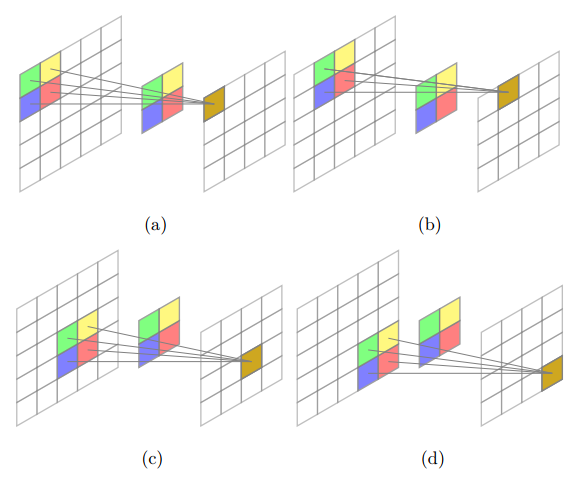
\includegraphics[width=0.8\textwidth]{convolution}
    \caption{Proces konvolucije}
    \label{fig:convolution}
\end{figure}

\section{Primjer konvolucijske mreže}
Nizanjem konvolucijskih slojeva dobivamo arhitekturu u kojoj se odgovornost filtera raspoređuje tako da je svaki sloj zadužen za jednostavniji potproblem sljedećeg sloja. Prvi slojevi uče atome poput linija, boje ili orijentacije čijim kombiniranjem je moguće raspoznati sve složenije geometrijske oblike. Na slici \ref{fig:dnn} prikazana je duboka neuronska mreža s 5 konvolucijskih slojeva među kojima se odvija sažimanje maksimalnom vrijednošću te dva sloja potpune povezanosti.
\newline

\begin{figure}[H]
    \centering
    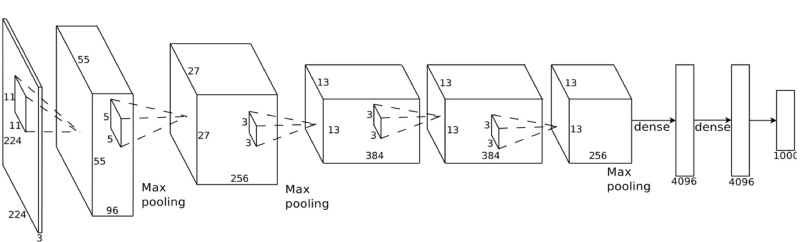
\includegraphics[width=0.9\textwidth]{dnn}
    \caption{Primjer duboke neuronske mreže}
    \label{fig:dnn}
\end{figure}


%%
% 	GENERATIVE MODELLING
%%


\chapter{Generativno modeliranje}
\section{Generativni naspram diskriminativnih algoritama}
Algoritme za učenje dijelimo na dvije temeljne skupine -- diskriminativne i generativne:
\newline

% setting item mark to bullet
\renewcommand{\labelitemi}{\textbullet}
\begin{itemize} 
\item Diskriminativni modeli baziraju se na modeliranju isključivo pomoću ulaznih varijabli ($X$) koje direktno mapiraju na ciljne vrijednosti ($Y$) i time uče uvjetnu vjerojatnost $p(Y\mid X)$. Pošto se fokusiraju samo na mapiranju viđenih značajki u klase, ne stvaraju puno pretpostavki o podložnoj distribuciji, ali su vrlo ovisni o kvalitetnim podatcima.

\item Generativni modeli rješavaju inverzan problem -- kako dobiti neku značajku $X$ kada znamo kojoj klasi $Y$ pripada, tj. pokušavaju naučiti distribuciju pojedinih klasa $p(X\mid Y)$.
\newline
\end{itemize}

Drugim riječima, dok diskriminativni modeli pokušavaju pronaći granicu između klasa, generativni modeliraju distribucije pojedinih klasa na temelju kojih mogu uzorkovati nove primjere.
\newline

\newpage
\section{Suparnički modeli}
Iako je očito da su generativni algoritmi svestranije naravi od diskriminativnih, u praksi se pokazalo kako diskriminativni modeli postižu bolje rezultate od generativnih. Sposobnost generalizacije dolazi s neizbježnim povećanjem složenosti koja proizlazi iz toga što se pronalazak ciljne distribucije u dubokim hijerarhijskim podatcima sastoji od rješavanja problema koje matematički nije moguće izvesti \cite{goodfellow2014generative}. Približna rješenja dobivena su uvođenjem mnogobrojnih aproksimacija, no nažalost, posljedica toga je da optimum dobivenog modela nikad neće biti dobar kao što bi bio onaj s pravim rješenjem.
\newline

Alternativni pristup ponuđen je u obliku suparničkih modela -- probleme kojima ljudi ne mogu pronaći rješenje, kroz dovoljno velik broj iteracija, moguće je naučiti pomoću dva modela koji se natječu u traženju čim bolje njegove aproksimacije dok ne pogode pravo rješenje. Ovisno o implementaciji, mreža takve arhitekture u stanju je izvesti distribuciju širokog spektra podataka: slika, govora, muzike, pa čak i pisanih zapisa.
\newline



\section{Rad generativnih suparničkih modela}
Ideja generativnih suparničkih modela bazirana je na učenje mreža kroz minimax igru -- umjesto izravnog rješavanja optimizacijskog problema, GAN sadrži funkciju kojoj mreže paralelno podešavaju ulaze dok ne dođu do stabilne točke u odnosu na maksimum jedne, a minimum strategije druge mreže. 
\newline

Pola mreže (generator $G$) bavi se stvaranjem novih podataka iz neke jednostavne distribucije $Z$ s ciljem da stvoreni podatci budu čim sličniji stvarnima. 

Paralelno s njegovim radom, druga polovica (diskriminator $D$) pokušava evaluirati koliko su uzorci $G(Z)$ slični stvarnim podatcima $Y$. Drugim riječima, dok $G$ pokušava minimizirati izlaz $D-a$, $D$ ga pokušava maksimizirati.
\newline
\newpage

Koraci rada GAN-a:
\begin{enumerate} 
\item Generator $G$ iz nasumičnih brojeva (šum) $Z$ stvara sliku $G(Z)$
\item Ta slika se zajedno sa uzorcima skupa stvarnih podataka $Y$ dovodi na ulaz diskriminatora $D$
\item Diskriminator $D$ određuje postotak vjerojatnosti da je slika $G(Z)$ prava
\end{enumerate}

\begin{figure}[H]
    \centering
    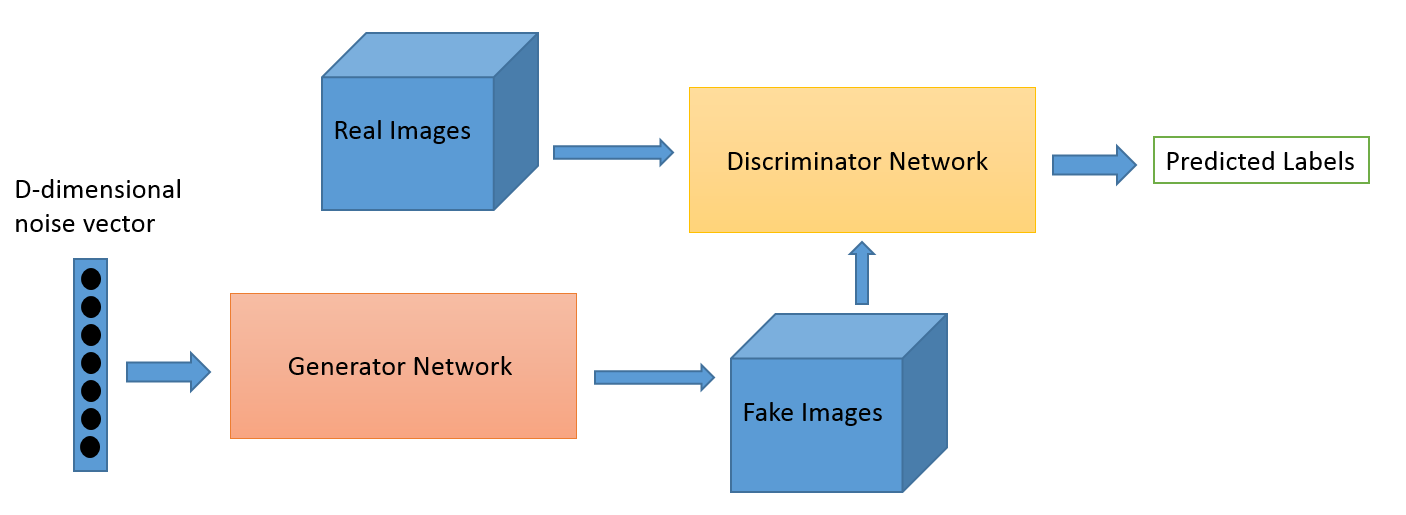
\includegraphics[width=0.9\textwidth]{gan_schema}
    \caption{GAN \cite{goodfellow2016nips}}
    \label{fig:convolution}
\end{figure}

\section{GAN-ovi naspram autoenkodera}
Uz GAN-ove, podjednako važna skupina generativnih modela su autoenkoderi. Ideja iza njihovog rada je da se sastoje od enkodera koji kompresira podatke u latentne varijable te dekodera koji iz tih varijabli ponovo generira ulaznu sliku. Naučenoj mreži možemo mijenjanjem latentnih varijabli vrlo precizno zadati kakve podatke želimo generirati. To im je ujedno i glavna prednost nad GAN-ovima koji generiraju dosta nasumične uzorke (što se može popraviti uz izmjene koje ću obraditi u sljedećim poglavljima).

Negativna strana varijabilnih autoenkodera je što uzorci koje proizvode imaju dosta anomalija što na slikama rezultira time da više nalikuju na umjetničke slike nego realnu reprezentaciju. Zbog toga primarnu primjenu nalaze u industrijama poput video igara i kompresiji podataka. U istraživanju su i mreže koje ujedinjuju te dvije tehnologije trenirajući dekoder pomoću GAN-a [larsen2015autoencoding].

\begin{figure}[H]
    \centering
    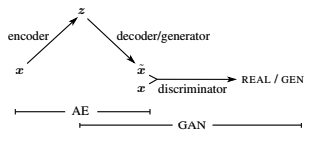
\includegraphics[width=0.7\textwidth]{vae-gan}
    \caption{Kombinacija autoenkodera i GAN-a}
    \label{fig:vae-gan}
\end{figure}


%%
% 	CONDITIONAL GANS
%%


\chapter{Uvjetne generativne mreže}
Kao što je spomenuto u prošlom poglavlju, jedna od većih mana generativnih suparničkih mreža je što generiraju poprilično nasumične uzorke. Pošto većina problema u praksi zahtijeva kontrolu nad tim procesom, jedno od najranijih proširenja GAN-ova vezano je upravo uz kontrolu generiranja podataka. 

Postavljanjem uvjeta na ulaz generativnog modela, moguće je usmjeriti generativni proces. Vrste uvjeta mogu biti raznolike: oznake klasa, skice, dubinske mape pa čak i cijele slike.

\begin{figure}[H]
    \centering
    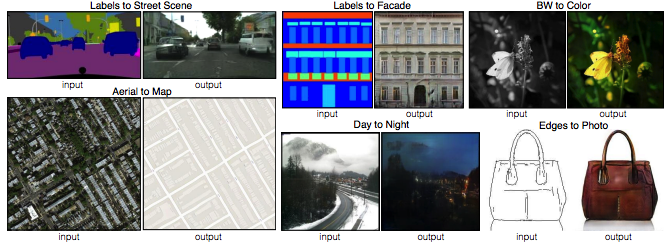
\includegraphics[width=1\textwidth]{isola2017-conditioned-generation}
    \caption{Primjeri uvjetovane generacije}
    \label{fig:isola2017-conditioned-generation}
\end{figure}


\section{Generalizacija problema prevođenja slike}
Jedan način razmatranja slika je kao višeslojni podatak u kojem se osnovni sadržaj obogaćuje raznolikim stilovima i načinima reprezentacije. 
Jednako kao što riječ možemo prevesti na više jezika zadržavajući određeni kontekst, ista scena može se prikazati kao dubinska mapa, RGB slika ili semantička segmentacija. Sukladno toj ideji, mnoge probleme procesiranja slika moguće je svesti na translaciju slike u drugačiju reprezentaciju. Neovisno radi li se o uklanjanju anomalija, ispravku boja ili izmjeni pozadine, u srži tih procesa može se prepoznati jedinstven problem: pronaći funkciju preslikavanja piksela u piksel. Vođeni time, Isola et al. osmislili su uvjetne generativne mreže kao generalno rješenje problema prevođenja slike \cite{isola2017image}.
\newline

\section{Pristup uvjetovanog prevođenja slike}
Zadavanje cilja neuronskim mrežama, a time i uspjeh njihovog učenja u potpunosti je bazirano na formulaciji funkcije gubitka. Lošim definiranjem te funkcije, neovisno o količini raspoloživih resursa i tipu mreže, nikad nećemo dobiti realistične rezultate. U GAN-ovima je ona zadana dosta općenito -- jesu li generirani podatci različiti od stvarnih uzoraka. Takva definicija omogućuje joj da se prilagodi podatcima te kao takva omogućuje generalizaciju nad setovima problema koji bi u suprotnom zahtijevali vrlo drugačije formulacije gubitka. 

Dok standardni GAN-ovi odbacuju sva rješenja koja se mogu razlikovati od stvarnosti generirajući slike $y$ iz nasumičnog šuma $z$ : $G: z \rightarrow y$, uvjetovani GAN-ovi dodatno usmjeravaju dobra rješenja prema željenoj distribuciji značajki dodavanjem uvjeta $x$ na šum $z$: $G: {x,z} \rightarrow y$ \cite{isola2017image}.

\section{Funkcija gubitka}
Kako su GAN-ovi sastavljeni od dvije mreže, za njihovo učenje potrebne su zasebne definicije funkcije gubitka. U slučaju neuvjetovanog GAN-a, $G$ ima cilj minimizacije $log(1 - D(G(z)))$ s obzirom na $D$ koji pokušava minimizirati $log(D(x))$.
Zajednička funkcija gubitka 

$ \Lagr_{GAN}(G, D) = \sum_{y}[log D(y)] + \sum_{x,z}[log(1 - D(G(x,z)))]$
\newline
koristi se za učenje kroz cilj mini-max igre:

$ G* = arg min_G max_D \Lagr_{GAN}(G, D)$.
\newline

Uvjetovanjem dodatnim informacijama $y$ na obje mreže taj cilj mijenja se u : 

$ \Lagr_{cGAN}(G, D) = \sum_{x,y}[log D(x,y)] + \sum_{x,z}[log(1 - D(x, G(x,z)))]$


%%
% 	UNPAIRED IMAGE TRANSLATION
%%


\chapter{Translacija bez uparenih primjera za učenje}
Učenje GAN-ova iz prethodnih poglavlja, kao i mnogih drugih algoritama, ovisi o postojanju velikih podatkovnih skupova označenih parova slika. S obzirom na to da izrada tih skupova iziskuje veliku količinu vremena i manualnog ljudskog rada, u mnogim slučajevima nam oni nisu dostupni.

\begin{figure}[H]
    \centering
    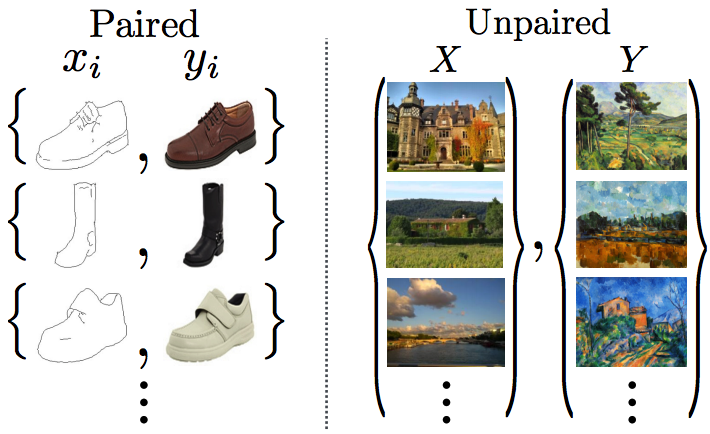
\includegraphics[width=0.7\textwidth]{zhu2017unpaired-paired-vs-unpaired}
    \caption{Parovi podataka (lijevo) ${\{x_i,y_i\}}_{i=1}^N$ te neupareni setovi (desno). }
    \label{fig:zhu2017unpaired-paired-vs-unpaired}
\end{figure}

\section{Kružni GAN-ovi}
Iako učenje bez označenih primjera izgleda kao poprilično drugačiji problem nego kad su prisutni, osnovni cilj ostaje isti -- naučiti preslikavanje s izvorišne domene $(X)$ na ciljnu $(Y)$: $G: X\rightarrow Y$ takvo da nije moguće razlikovati distribuciju $G(X)$ od distribucije $Y$. 

Kompleksnost proizlazi iz toga što je taj cilj vrlo nespecifičan, a bez primjera koji bi pružali smjernice tijekom učenja rezultati su nekonzistentni i previše raznoliki da bi bili primjenjivi.

Kružni GAN-ovi zato uvode uvjet tranzitivnosti nad ciljnom funkcijom kao način regularizacije u svrhu provođenja dosljednosti ponašanja modela.
Definirajući inverz funkcije $G$: $F: Y \rightarrow X$, funkciju gubitka osnovnog GAN-a proširuju gubitkom cikličke dosljednosti: $F(G(X)) \approx X$.

\begin{figure}[H]
    \centering
    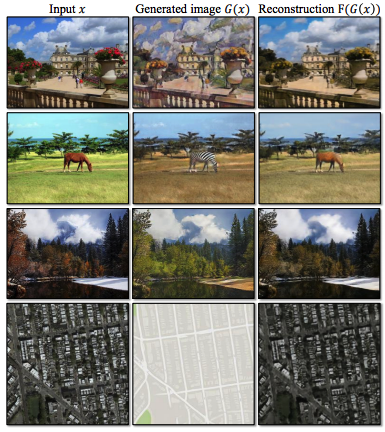
\includegraphics[width=0.7\textwidth]{zhu2017unpaired-reconstruction}
    \caption{Primjeri nenadziranog GAN-a s i bez rekonstrukcije}
    \label{fig:zhu2017unpaired-reconstruction}
\end{figure}

Oslanjajući se na pretpostavku da izvorišna i ciljna domena nisu u potpunosti nasumične nego sadrže podložnu zajedničku distribuciju, inverzom pretvaraju ovaj problem u nadzirano učenje. Pri tome umjesto značajki iz parova primjera, uče zajedničke specifičnosti cijelih setova te njih koriste za nadziranje.

\subsection{Gubitak cikličke dosljednosti}
Iako suparničke mreže u teoriji mogu naučiti preslikavanja $G$ i $F$ koja stvaraju uzorke jednake distribucije kao $Y$ i $X$, u praksi često nauče samo preslikavanje na podskup uzoraka ciljne domene. Iz tog razloga, gubitak suparničke mreže 


\begin{equation}
\begin{split}
\Lagr_{GAN}(G, D) &= \sum_{y\sim p_{data(y)}}[log D(y)] \\
			     &+ \sum_{x\sim p_{data(x)}}[log(1 - D(G(x)))]
\end{split}
\end{equation}

nije dovoljno specifičan da osigura željenu translaciju slike.
\newline

Kako bi smanjili prostor mogućih funkcija preslikavanja, cikličkom dosljednošću forsiramo da dvosmjerni ciklus translacije mora izvornu sliku $x \in X$ preko translatirane $y \in Y$ preslikati nazad u izvornu reprezentaciju: $x \rightarrow G(X) \rightarrow F(G(x)) \approx x$. (Isto vrijedi u obrnutom smjeru.)

\begin{equation}
\begin{split}
\Lagr_{cyc}(G, F) &= \sum_{x\sim p_{data(x)}}[ \parallel F(G(x)) - x \parallel ] \\
			   &+ \sum_{y\sim p_{data(y)}}[ \parallel G(F(y)) - y \parallel ]
\end{split}
\end{equation}

\subsection{Prednosti}



\newpage
\section{Multimodalna translacija (MUNIT)}
Poveća mana spomenutih načina translacije je manjak raznolikosti u translatiranim izlazima. One ne uzimaju u obzir da je uvjetna distribucija preslikavanja slika između dvije domene inherentno multimodalna \cite{huang2018multimodal} što kao posljedicu ima da pri generiranju vrlo teško stvaraju vidljivo različite uzorke. MUNIT model pretpostavlja da se reprezentacija slike može rastaviti na značajke koje su domenski invarijantne te na one koje sadrže domenski specifična svojstva. Zatim se pri generiranju jednostavno domenski invarijantne značajke kombiniraju s nasumičnim stilskim kodom uzorkovanim s ciljne domene.
\newline

Pri podjeli reprezentacija sadržaja i stila, sadržaj se odnosi na prostornu strukturu dok je stil ograničen na rendering te strukture.
%A concurrent work also recognizes this limitation and propose an extension of CycleGAN for multimodal mapping \cite{almahairi2018augmented}


\chapter{Prijenos stila}
Cilj prijenosa stila je modificiranje stilističke perspektive slike uz očuvanje sadržaja. Generalna podjela metoda ovog procesa dijeli ih na prijenos na temelju primjera te na prijenos zajedničkog stila neke kolekcije. Dok se klasični pristupi baziraju na prvoj skupini, neuronske mreže bolje rezultate postižu na drugoj.

\section{Očuvanje strukture}
Postojeće metode ograničene su izborom stilova koje mogu prenijeti te u realističnosti dobivenih rezultata. Pokušaji prijenosa stila koji mijenjaju vrijednost piksela unose sitne izmjene u linijama i teksturama što na rezultantnom sadržaju stvara dojam crteža, a gubi se realističnost fotografije. Uvjet koji se zbog toga postavlja na rad mreže je da može unositi izmjene isključivo na prostoru boja.

\section{Lokalizacija stila i očuvanje konteksta} \cite{luan2017deep}
Postoji još jedan faktor koji povećava kompleksnost cijelog procesa, a to je da se ciljano ponašanje prijenosa stila drži konteksta izmjene. Na primjer, ako se na fotografiji nalaze livada i oblaci, modifikacije na livadi moraju biti povezane sa stilom livade na referentnoj slici, a ne da povuku stil s oblaka. 


%%
% 	CONCLUSION
%%


\chapter{Zaključak}
Generativni modeli tema su mnogobrojnih istraživanja i vrlo obećavajuća metoda učenja 'prirodnih' značajki podataka. Uz napretke koji se redovno postižu u njihovom unaprjeđenju, velika je vjerojatnost da će ubrzo biti u stanju generirati uzorke nerazlučive od stvarnosti. Time primjenu pronalaze u područjima poput stvaranja virtualnih svjetova bez ljudske intervencije, izvršavanja modifikacija nad slikama pomoću jednostavnog govora, regeneriranju oštećenih podataka ili stvaranju novih za buduća istraživanja.
\newline

...
Uvjetnim suparničkim mrežama pokazano je da osim što više nije potrebno ručno izvoditi funkcije preslikavanja, zadovoljavajuće rezultate možemo dobiti i ako dubokoj mreži prepustimo da sama nauči funkciju gubitka. To je velik korak prema široj adaptaciji ove tehnologije upravo zato što uklanja potrebu za inženjerom i omogućava ljudima poput umjetnika i mladih znanstvenika da ju koriste samostalno.
...
\newline

\bibliographystyle{fer}
\bibliography{literatura}


\begin{sazetak}
Mnogi problemi u procesiranju slika odnose se na translaciju ulazne slike u željenu izlaznu. Većina današnjih arhitektura bazira se na generativnim suparničkim mrežama, nad kojima su osmišljena mnoga proširenja kako bi se prilagodila specifičnim problemima. Uvjetnim generativnim mrežama nije potrebno definirati funkciju gubitka jer ju mogu same naučiti, kružne generativne mreže sposobne su učenju translacije ne samo ulaznih u izlazne primjere nego i u drugom smjeru, a ograničavanjem mreže na translaciju unutar prostora boja obavljat će prijenos stila bez distorzije sadržaja slike. Ovim radom usporedit ću različite arhitekture, njihove karakteristike i primjene na problemima translacije slike u sliku.

\kljucnerijeci{image-to-image generation, style transfer, GANs, CycleGANs}
\end{sazetak}

\engtitle{Image to image generation using CycleGANs}
\begin{abstract}

\keywords{image-to-image generation, style transfer, GANs, CycleGANs}
\end{abstract}

\end{document}